%
% 02_Naiver_weg.tex -- Beispiel-File für das Paper
%
% (c) 2020 Prof Dr Andreas Müller, Hochschule Rapperswil
%
% !TEX root = ../../buch.tex
% !TEX encoding = UTF-8
%
\section{Herleitung
\label{schwimmen:section:naiver_weg}}
\kopfrechts{Herleitung}

Hier ist eine Schritt für Schritt Darstellung der Herleitung zur
optimalen Flussüberquerung dargestellt. Als Inspiration der Bilder
und der Herangehensweise wurde an die Forumsfrage in
\cite{schwimmen:mathForum} angelehnt.

%
% fig-quadratisch.tex
%
% (c) 2024 Prof Dr Andreas Müller
%
\begin{figure}
    \centering
    %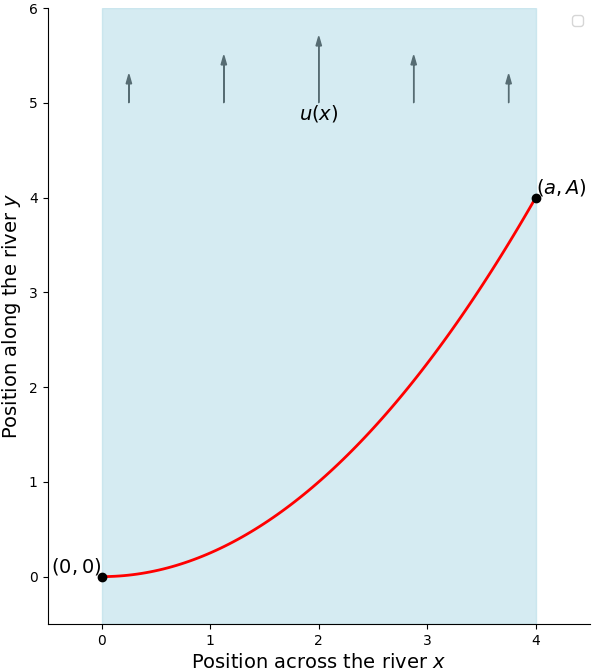
\includegraphics[width=0.6\textwidth]{papers/schwimmen/Grafiken/Figure_1-crop.png}	
    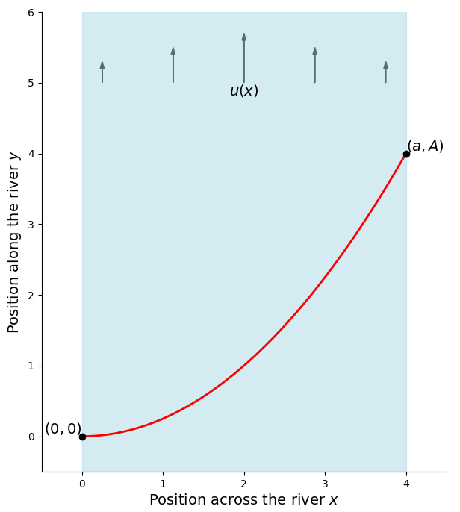
\includegraphics{papers/schwimmen/tikz/quadratisch.pdf}
    \caption{Fluss mit quadratischer Strömung. Ziel ist es von Punkt \((0,0)\)
    zum Punkt \((a,A)\) zu kommen, der am anderen Ufer liegt.}
    \label{fig:river_template}
\end{figure}
%

Ziel ist es die schnellste Route über den Fluss zu finden. In
Abbildung \ref{fig:river_template} ist eine Flussüberquerung
abgebildet, wobei \(a\) die Flussbreite ist und \(A\) die Distanz
entlang des Flusses. Im Falle unserer Aufgabenstellung ist \(A=0\),
da man am andern Ufer auf gleicher Höhe ankommt.

\subsubsection{Wichtige Kenngrössen}
Ein paar wichtige Kenngrössen für die Herleitung sind in Tabelle
\ref{table:Wichtige_Kenngroessen} zufinden.

\begin{table}
    \centering
    \renewcommand{\arraystretch}{1.3}
    \begin{tabularx}{\textwidth}{@{}ll>{\raggedright\arraybackslash}p{7cm}@{}}
        \multicolumn{3}{c}{Wichtige Grössen} \\
        % \specialrule{.1em}{.05em}{.05em}
        % \textbf{Dataset} & \textbf{\(\mu\) in \(\mathrm{ps}\)} & \textbf{\(\sigma\) in \(\mathrm{ps}\)} \\
        \hline
        \(a\)   &   Flussbreite  &   definiert von der Umgebung \\
        \(c\)   &   Schwimmgeschwindigkeit        &   Definiert von der schwimmenden Person       \\
        \(u(x)\)   &   Flussgeschwindigkeit         &   Ist von der \(x\)-Position im Fluss abhängig     \\
        \((0,0)\)   &   Startpunkt         &   Startpunkt am Flussufer     \\
        \((a,A)\)   &   Endpunkt         &   Endpunkt auf anderer Ufer aber auf gleicher Höhe     \\
        %\specialrule{.1em}{.05em}{.05em}
	\hline
    \end{tabularx}
    \caption{Wichtige Kenngrössen für die Herleitung}
    \label{table:Wichtige_Kenngroessen}
\end{table}


\subsubsection{Schwimmgeschwindigkeiten}
\index{Schwimmgeschwindigkeit}%
Als erstes werden die Geschwindigkeiten der schwimmenden Person
definiert. Mittels den Schwimmrichtungsvektoren und dem Flussvektor
können folgende Geschwindigkeiten für die in \(x\)- und \(y\)-Richtungen
geschwommenen Geschwindigkeiten relativ zum Ufer genommen werden:
\begin{align*}
    c_x &= c\cdot \cos(\theta)
\label{eq:c_x_equation}
\\
    c_y &= u(x) + c \cdot \sin(\theta).
%\label{eq:c_y_equation}
\end{align*}
\(c_x\) ist die Geschwindigkeit in \(x\)-Richtung der schwimmenden
Person, \(c_y\) ist die Geschwindigkeit in \(y\)-Richtung wie auch
die Flussgeschwindigkeit. Dabei ist der Winkel \(\theta\) der
Schwimmwinkel in Bezug auf die \(x\)-Richtung.


\subsubsection{Zeitoptimierung}

Für den geringsten Energiekonsum wird die Zeit optimiert. Die Zeit
kann durch folgendes Integral dargestellt werden:
\begin{equation}
    T = \int_0^a\,dt \label{eq:Time_river_1}.
\end{equation}
Da \(dt = \frac{dx}{c_x}\), die Zeit, die benötigt wird um sich ein
kleines Stück in \(x\)-Richtung zu bewegen, von der Geschwindigkeit
in \(x\)-Richtung abhängt, kann man \eqref{eq:Time_river_1} erweitern
zu

\begin{equation*}
    T = \int_0^a\,dt = \int_0^a\frac{dx}{c\cdot \cos(\theta)}.
%\label{eq:Time_river_2}
\end{equation*} 


\subsubsection{Beziehung der \(x\)- und \(y\)-Geschwindigkeiten}

Als nächstes wird die Beziehung der \(x\)- und \(y\)-Geschwindigkeiten
im System behandelt. Dies ist auch am Schluss wichtig, um den genauen
Schwimmverlauf der schwimmenden Person beobachten zu können.

Die \(y\)-Geschwindigkeit soll im Bezug zur \(x\)-Richtung gegeben
werden. Die Schwimmgeschwindigkeit in \(y\)-Richtung ist gegeben
durch
\begin{equation*}
    c_y = \frac{dy}{dt}.
\end{equation*}
Darauf kann die Kettenregel angewendet werden, um
\begin{equation*}
    \frac{dy}{dt} = \frac{dy}{dx} \cdot \frac{dx}{dt} = \frac{dy}{dx}\cdot c_x = \frac{dy}{dx}\cdot c\cdot \cos(\theta)
\end{equation*}
zu bekommen. Mittels \(c_y = u(x) + c\cdot \sin(\theta)\) bekommt man die Beziehung der \(x\)- und \(y\)-Geschwindigkeiten:
\begin{equation}
\frac{dy}{dx}
=
\frac{u(x) + c \cdot \sin(\theta)}{c \cdot \sin(\theta)}.
\label{eq:dy_dx}
\end{equation}



\subsubsection{Auflösen nach \(\theta\)}

Der letzte Schritt für das Aufstellen die Integrals ist es, eine
Formel für den Winkel \(\theta\) zu haben.
Ausgehend von \eqref{eq:dy_dx} können die Umformungen  
\begin{align*}
    \frac{dy}{dx} &= \frac{\dot{y}}{\dot{x}} = \frac{c_y}{c_x} = \frac{u(x) + c \cdot \sin(\theta)}{c \cdot \sin(\theta)} \\
    \frac{dy}{dx} &= \frac{u}{c}\cdot \sec(\theta) + \tan(\theta) \\
    \frac{dy}{dx} &= \frac{u}{c}\cdot \sec(\theta) + \sqrt{\sec^2(\theta)-1}
\end{align*}
gemacht werden. Dabei sind folgende Formeln für die Umformungen zu
beachten: \[\frac{1}{\cos(\theta)} = \sec(\theta)\] und
\[
\sec^2(\theta)-\tan^2(\theta) = 1.
\]
Durch Quadrieren und aus
\[
\frac{dy}{dx} = y'
\]
folgt
\begin{equation}
    \biggl(\frac{u^2}{c^2}-1 \biggr) \cdot \sec^2(\theta) - \frac{2uy'}{c}\cdot \sec(\theta) + y'^2 +1 = 0
\label{eq:gleichung_pre_quad}
\end{equation}
als Gleichung. Als Lösung der quadratischen Gleichung
\eqref{eq:gleichung_pre_quad} bekommt man mit der bekannten
Lösungsformel
\begin{equation*}
    \sec(\theta)
    =
    \frac{
		\displaystyle
		\frac{2uy'}{c} \pm \sqrt{4\biggl(y'^2-\frac{u^2}{c^2} + 1\biggr)}
	}{
		\displaystyle
		2\biggl(\frac{u^2}{c^2}-1\biggr)
	}
\end{equation*}
für den Winkel \(\theta\). Durch weiteres Umformen bekommt man
\begin{equation}
    \frac{1}{c}\cdot \sec(\theta) = \frac{-uy' \mp \sqrt{c^2(y'^2+1)-u^2}}{c^2-u^2} .
\label{eq:theta_1}
\end{equation}


\subsubsection{Zeitintegral}

Nun kann man die Formel \eqref{eq:theta_1} für den Winkel, in das Zeitintegral einfügen:
\begin{equation}
    T = \int_0^a\,dt = \int_0^a\frac{dx}{c\cdot \cos(\theta)} = \int_0^a \frac{-uy' \mp \sqrt{c^2(y'^2+1)-u^2}}{c^2-u^2} \,dx.
    \label{eq:Time_river_2} 
\end{equation}
Dieses Integral beschreibt die Zeit, die für die Flussüberquerung benötigt wird. 



\subsubsection{Lagrange-Funktion} 
Um die Route zu finden, die die kürzeste Zeit für die Flussüberquerung
benötigt, wendet man die Variationsrechnung an. Dafür braucht man
das  Funktional, welches minimiert werden soll, in diesem Fall
\eqref{eq:Time_river_2}.
Aus dem Funktional \eqref{eq:Time_river_2} kann die Lagrange-Funktion
\begin{equation*}
    L(x, y, y') = \frac{-uy' \mp \sqrt{c^2(y'^2+1)-u^2}}{c^2-u^2}
%\label{eq:lagrange_integral}
\end{equation*}
herausgelesen werden. 

\subsubsection{Euler-Lagrange-Differentialgleichung}
Die Euler-Lagrange-Differentialgleichung kann vereinfacht werden,
da sie nicht direkt von \(y\) abhängig ist:

\begin{align*}
    \frac{\partial L}{\partial y} - \frac{d}{dx}\frac{\partial L}{\partial y'} = 0 - \frac{d}{dx}\frac{\partial L}{\partial y'} &= 0 \\
    \frac{d}{dx}\frac{\partial L}{\partial y'} &= 0.
\end{align*}
Daraus folgt die Ableitung der Lagrange-Funktion:
\begin{figure}
    \centering
    \begin{subfigure}{0.48\textwidth}
        \centering
        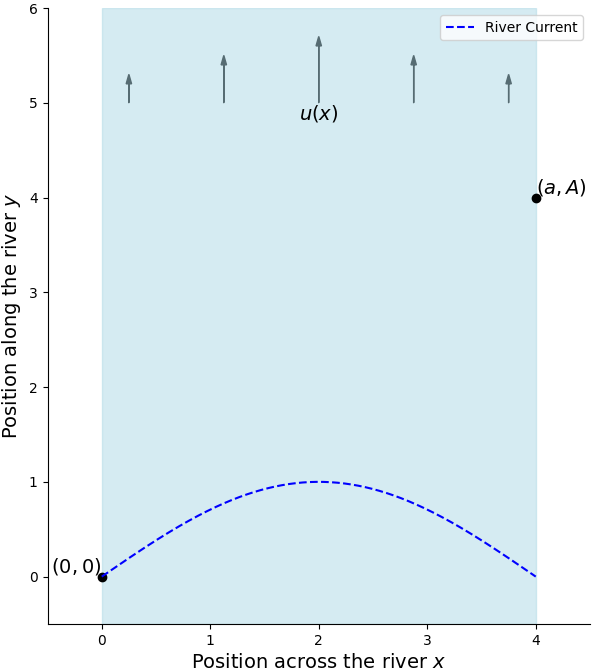
\includegraphics[width=\textwidth]{papers/schwimmen/Grafiken/Figure_2-crop.png}	
        \caption{Flussströmung}
        \label{fig:no_velocity}
    \end{subfigure}
    \hfill  
    \begin{subfigure}{0.48\textwidth}
        \centering
        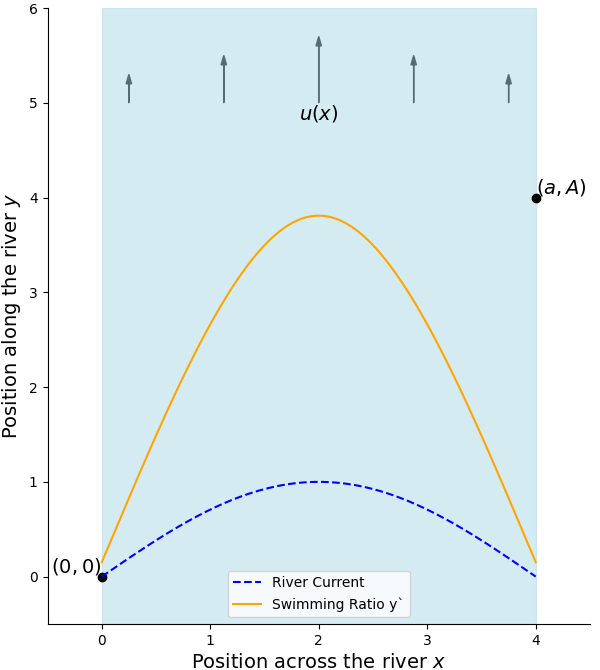
\includegraphics[width=\textwidth]{papers/schwimmen/Grafiken/Figure_3-crop.png}	
        \caption{\(y' = \frac{dy}{dx}\)}
        \label{fig:diagonal_velocity}
    \end{subfigure}
    \par\bigskip
    \begin{subfigure}{0.48\textwidth}
        \centering
        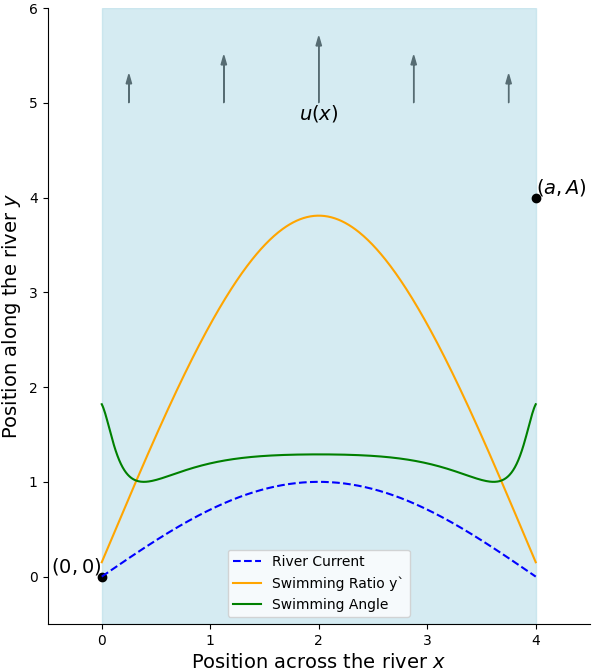
\includegraphics[width=\textwidth]{papers/schwimmen/Grafiken/Figure_4-crop.png}	
        \caption{Winkel der Schwimmenden Person}
        \label{fig:squerd_velocity}
    \end{subfigure}
    \hfill  
    \begin{subfigure}{0.48\textwidth}
        \centering
        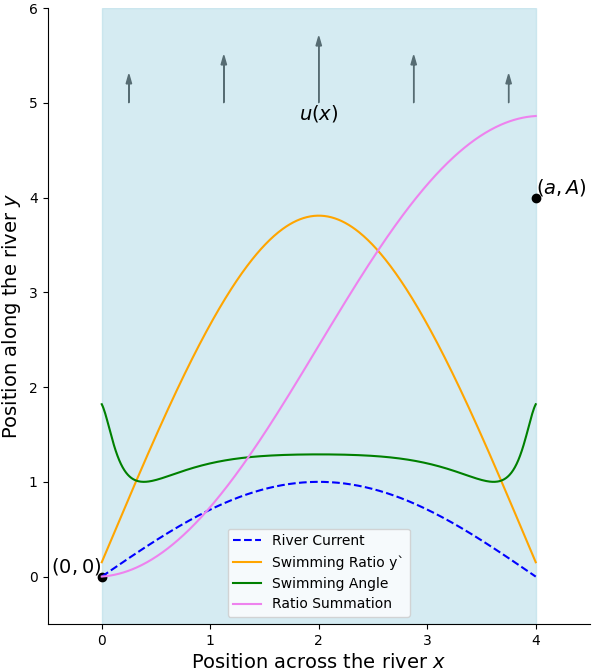
\includegraphics[width=\textwidth]{papers/schwimmen/Grafiken/Figure_5-crop.png}	
        \caption{Aufsumierte Steigung}
        \label{fig:sin_velocity}
    \end{subfigure}
    \par\bigskip
    \caption{Die vier Grafiken stellen verschiedene Graphen dar die für die Flussüerquerung zentrall sind, (a) stellt die Flussströmung dar, (b) das Verhältis zwischen was in \(x\)- und \(y\)-Richtung geschwommen wird, (c) den Winkel der aus dem Verhältnis folgt und (d) das aufsummierte Verhältnis}
    \label{fig:river_pfrofiles}
\end{figure}
%
\begin{align*}
    \frac{\partial L}{\partial y'} &= \text{constant}
%\label{eq:Lagrange_derivites_1}
\\
    \frac{\partial L}{\partial y'} &= \frac{\partial}{\partial y'} \biggl (\frac{-uy' \mp \sqrt{c^2(y'^2+1)-u^2}}{c^2-u^2}\biggr) \\
    &= \frac{c^2\cdot y'}{\sqrt{c^2(y'^2-u^2)}(c^2-u^2)} - \frac{u}{c^2-u^2} \\
    &=  \frac{1}{c^2-u^2} \biggl( \frac{c^2\cdot y'}{\sqrt{c^2(y'^2-u^2)}} - u \biggr ) \\
    &= \text{constant} = \frac{1}{g}.
%\label{eq:Lagrange_derivites_2}
\end{align*}
Auflösung nach \(y'\) ergibt
\begin{equation}
    y' = \frac{c^2 + g\cdot u - u^2}{c \cdot \sqrt{u^2-2\cdot g\cdot u - c^2 + g^2}} .\label{eq:angle} \\
\end{equation}
\(y'\) gibt an, mit welchem Verhältnis von \(y\) zu \(x\) sich die
schwimmende Person im Wasser bewegt. Die rechte Seite von
\eqref{eq:angle} ist eine Funktion nur von \(x\), nicht von \(y\).
Daher kann die Route durch die Integration
\begin{align*}
    y(x) &= \int_0^x y'(\xi) \,d\xi \\
    &= \int_0^x \frac{c^2+g\cdot u(\xi) - u(\xi)^2}{c\cdot \sqrt{u^2 - 2\cdot g \cdot u(\xi) - c^2 + g^2}} \,d\xi
\end{align*}
gefunden werden. Die Konstante \(g\) muss so gewählt werden, dass
\(y(a) = A\), d.h. dass die schwimmende Person am gewünschten Zielort
ankommt.


